\section{Understanding polarization signatures of magnetized filaments}
% 
\begin{figure}[t]
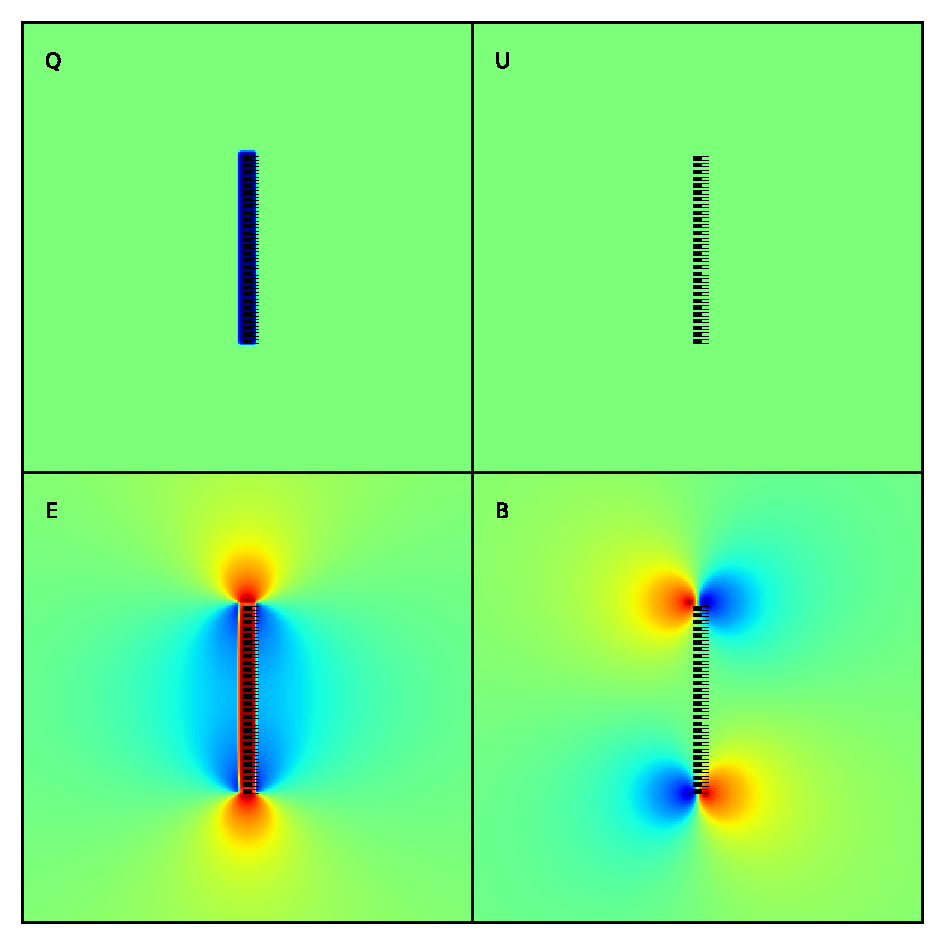
\includegraphics[width=0.5\columnwidth]{line.pdf}
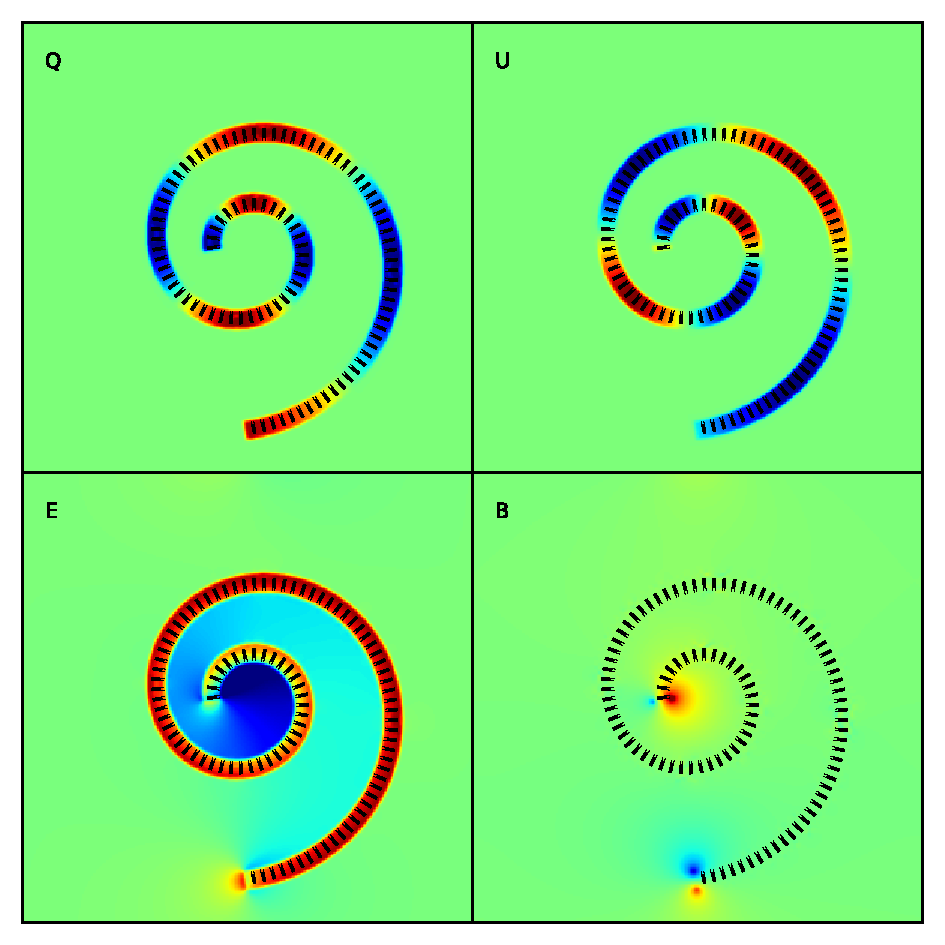
\includegraphics[width=0.5\columnwidth]{spiral.pdf}
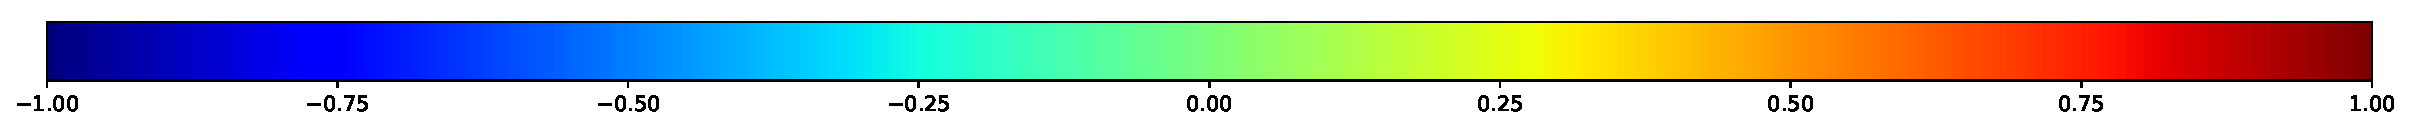
\includegraphics[width=1.0\columnwidth]{colorbar.pdf}
\caption{ The polarization signals of toy filament structures. In a filament organized perfectly along a magnetic field line, the polarization will be perpendicular to the filament direction.  The $E/B$ modes of filaments are in some ways easier to think about than the Stokes parameters. Left panels: in a straight filament, the E-mode is positive along the filament and at the ends, but negative along the sides.  B-modes are only non-zero at the ends.  Right panels: in a curved filament, the E-mode is again positive along the filament.  Outside the filament, the $E$-mode is more negative on the interior of the curve than the exterior.  The $B$-modes are again non-zero only at the ends, and are akin to the straight filament case. In all images, the longitude angle increases to the left (which is East in sky convention).  All plot are on a common, arbitrary color scale.}
\label{fig:polfilaments}
\end{figure}
%

The real space kernels give us a better intuitive understanding of the $E/B$ modes associated with physical objects.  For example, a simple model for a magnetized filament has the magnetic field threaded along a linear gas overdensity.  Precession of the dust grains around the magnetic field leads to a net polarization perpendicular to the magnetic field (and perpendicular to the filament overall).  For a filament aligned North--South, the polarization will be horizontal or $Q<0$, $U=0$ (left pane of \fig{fig:polfilaments}).  The Green's function kernels for horizontal polarization are rotated by 90 degrees relative to the components of $\cal{M}_G$ in \fig{fig:vis_kernel}.

The kernel can be thought of as the orientable nib of a calligraphy pen or paintbrush that we can trace along the filament.  The positive components for the $E$ part of the Green's function align and reinforce along the filament, and so the filament is highlighted as a segment with $E>0$.  Since the overdensity will also have emission in total intensity, this naturally predicts a positive $TE$ correlation for magnetized filaments.  The $E$ pattern is somewhat negative along the outside of the filament, also a consequence of the kernel shape.

The $B$ part of the Green's function, traced along the filament, cancels itself except at the filament ends.  This results in a non-zero $B$ pattern for the filament.  For a North--South filament, the $B$-mode pattern is positive on the North-East and South-West, and negative in the North-West and South-East.  The size of this $B$-mode pattern is set by the dimensions of the filament, chiefly the width.

The non-zero $B$ result is somewhat surprising given that the polarization pattern is symmetric to both horizontal and vertical reflections through the filament center.  However, unlike a circular ring, this filament is not a configuration with a definite parity.  Since the scalar description of polarization is coordinate independent, the $E/B$ patterns do not depend on the orientation of the filament.  A filament inclined at $45^\circ$ will have a similarly inclined $E/B$ pattern, but different reflection symmetries.  

Changing the polarization direction within the filament changes the $E/B$ patterns.  A $90^\circ$ rotation of the polarization with respect to the filament changes the sign of both $E$ and $B$.  In a polarization pattern aligned at $45^\circ$ to the filament, the $E$ pattern will swap with the $B$ pattern.  The work in \cite{Zaldarriaga2001a} correctly argued that linear filaments (infinite and without ends) can only produce $E$-power, but we find that for realistic filaments, the ends produce $B$-mode power with a clear signature.  Careful study of the $E/B$ mode power in filaments can provide insights into the orientation of the magnetic field with respect to the length of the filament.

The intuition from the real-space kernels holds also when we distort the shape of the filament.  If the filament were bent around into a circle, the positive and negative parts of the $B$ pattern will cancel, and we are left with a hoop of pure $E$ pattern. Here it is important to note that this cancellation will not happen for an ellipse or any loop of non-contant radius of curvature.  The same general description holds for a spiral-shaped filament, which can can be viewed as distortion of the straight filament.  The filament is highlighted by positive $E>0$.  The $E$-pattern is more negative on the interior of a curve than on the exterior, and the concentric rings of filamentary structure make an increasingly negative $E$ value inside. While the $B$-pattern is again concentrated at the ends of the filament in an oriented pair of positive/negative fluctuations, note that it is non-vanishing in the intermediate regions along the filament due to the varying radius of curvature of the spiral.
%\footnote{ \revisit{Why do we use this specific spiral - Its easy to compute the tangent to the spiral at any point.}}.

%\comment{If this is correct, then one expects to see a higher B-mode signal in intermediate regions of the spiral, as compared to the B-mode signal in the intermediate regions of the linear filament. This  then should be more visible in a logarithmically scaled version of Fig. 8.}  % K: addressed with new plot

%\revisit{Note that we have made the simplifying assumption that the polarization headless vectors are perpendicular to the magnetic field which is always assumed parallel to the tangent to the filament at any given point. This results in generating dominantly an E-mode signal while the B-mode signal is present only near the edges. By similar arguments it can be shown that that polarization pattern will be dominated by B-modes if the polarization vectors were aligned at $+45$ (or $-45$) degrees to the tangent to the filament while the E-mode signal would only be present at the edges. One way to get this configuration is to change the orientation of the magnetic field vector with respect to the tangent to the filament. Therefore a careful study of the $E/B$ mode power in filaments can provide insights into the orientation of the magnetic field with respect to the length of the filament.} % K: addressed

%\revisit{A stacking analysis of Planck data \citep{2016A&A...586A.141P} sees $E>0$ along filaments (selected from intensity data), but no $B$-mode signal is above the noise.  We predict that it should be there in higher fidelity data.}
A stacking analysis of Planck data \citep{2016A&A...586A.141P} sees $E>0$ along filaments (selected from intensity data), but claim no $B$-mode signal above the noise. We predict that a B-mode signal from filaments should be present, since they have a finite length of a few degrees.  Detecting B-modes from filaments will be easier with more signal-to-noise and may require a more careful filament analysis, rescaling and aligning the filament ends.  The detectability of the $B$-mode signature from stacked filaments in Planck data calls for a more careful assessment, we should see it in higher-fidelity data.

%\revisit{In \cite{Zaldarriaga2001a} it is argued that linear filaments of infinite length in which the configuration of the polarization vector is parallel or perpendicular to the length of the filament cannot produce B-mode power. While this conclusion is true for filaments of infinite length, in reality we expect filaments that are observed on the sky to have a finite length and in this case one expects a definite B-mode pattern from the edges of the filament. One also does not expect that filaments have a constant radius of curvature and this will result in an additional generation of B-mode power. Therefore our study indicates results which subtly differ from those presented in \cite{Zaldarriaga2001a} and these differences can be attributed to the more realistic assumptions about the geometry of the filaments made in our analysis.} \comment{Move to conclusions?}
 

